\chapter{Motivation}
\label{motivation}
As described in \autoref{intro:clustering} intermolecular interactions of FAK molecules effect their activation. However, the process is still not understood, especially on an atomistic scale.\\
In this thesis we used MD simulations with the \martini{} force field to investigate these interactions. \martini{} lacks chemical details, but it is a necessary simplification since systems with several FAK molecules involve a large number of particles. Unfortunately, previous work in the group \autocite{sara} revealed problems in the use of \martini{} regarding simulations of FAK, which are summarized in the following.\\
\\
\textcite{sara} obtained in simulations of a single FAK molecule on a \pip{} containing membrane rapid changes in the inclination of the protein with respect to the membrane. In the following part, this inclination is characterized by the angle $\beta$ between the z-axis and the vector connecting F1 and F2, $\vec{d}_F$. $\beta$ is given as
\begin{equation}
\cos\left(\beta\right) = \frac{\vec{d}_{F, z}}{d_F},\quad d_F = \left|\vec{d}_F\right|
\end{equation}
The distributions of $\beta$ for different simulations ($10\,\si{\micro\second}$) are presented in \autoref{motiv:sarascurves}. The red line, for example, shows a mean value of $90\,\si{\deg}$. The angle changed in less than $50\,\si{\nano\second}$ and stayed constant for the remaining simulation time. We refer to this behaviour as a fall of FAK in the following.\\
There are several reasons why this is rather an artefact of the \martini{} force field than a possible binding pose of FAK to the membrane as suggested by \textcite{pap002}. First, FAK fell to both sides, which means that the interaction sites for \pip{} proposed by \textcite{pap002} were also located on top of the protein instead of at the protein membrane interface. Indeed, contact analysis between the protein and \pip{} lipids showed that virtually all residues on the surface (in both, FERM domain and kinase) were interacting with the membrane. A second reason is, that this behaviour was not observed in equivalent all atom simulations in \charmm{} ($1.5\,\si{\micro\second}$ in total). Here only two maxima were observed around $8\,\si{\deg}$ and around $20\,\si{\deg}$, the largest observed angle was $40\,\si{\deg}$.\\
\\
In the course of this project we carried out several experiments to understand the cause of this falling. However, we were not able to prove the reason beyond doubt. In order to still perform reasonable simulations of multiple FAK molecules, we decided to apply a stabilizing force on each FAK molecule.\\
The force is acting onto F1 and F2 parallel to the z-axis and is proportional to the deviation of their z-distance $\Delta z$ from a reference distance $z_0$. This is illustrated in \autoref{motiv:forceillustr}. For the determination of $z_0$ we took only the green and the blue distribution into account, because the large angles observed in the other distributions have not been observed in the \charmm{} simulations. The mean value of $\vec{d}_{F, z}$ for these two distributions is $2.228\,\si{\nano\metre}$, which we therefore set as $z_0$. From the standard deviation of $\vec{d}_{F, z}$, $\Delta z = 0.11\,\si{\nano\metre}$ we estimated the maximum force constant $k_m$, which does not sharpen the distribution.
\begin{equation}
	k_B T &= \frac{1}{2} k_m \Delta z^2
	k_m &= \frac{2 k_B T}{\Delta z^2} = 412 \frac{\si{\kilo\joule}}{\si{\mole} \si{nano\metre}^2}
\end{equation} 
We choose $k = 100 \frac{\si{\kilo\joule}}{\si{\mole} \si{nano\metre}^2}$.
%
%
%
\begin{figure}
	\subcaptionbox{\label{motiv:sarascurves}}[0.49\textwidth]{
		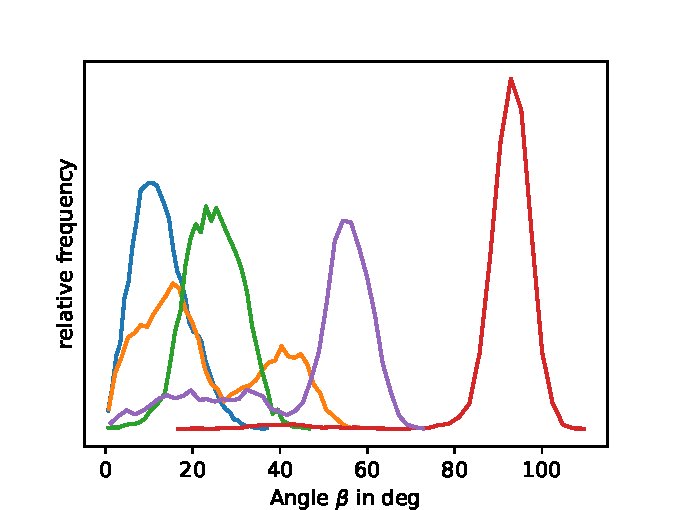
\includegraphics[height=5cm]{figures/introduction/sara_angles}
	}\hfill%
	\subcaptionbox{\label{motiv:forceillustr}}[0.49\textwidth]{
		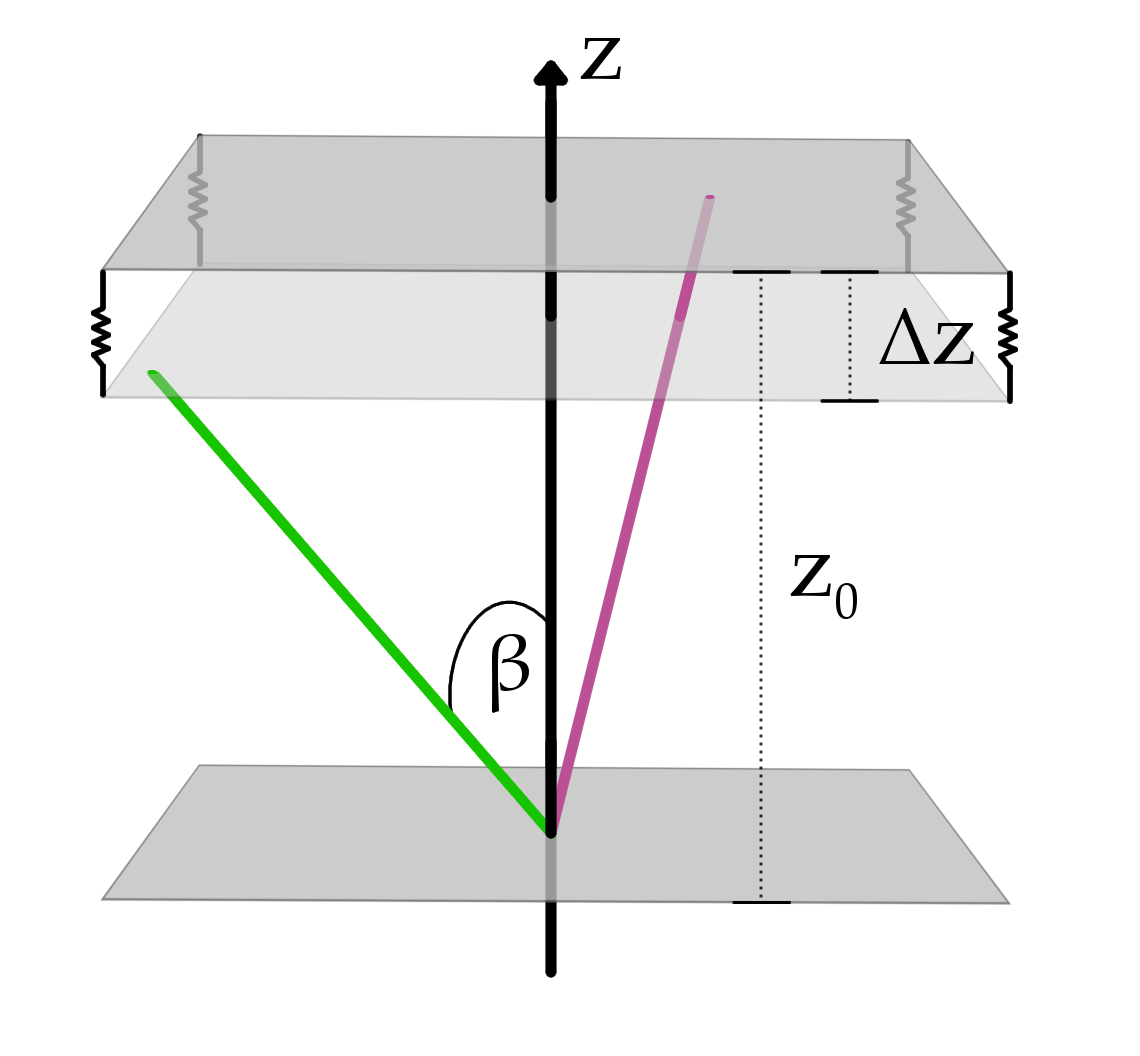
\includegraphics[height=5cm]{figures/introduction/forceapproach}
	}%
	\nicecaption{Inclination angle of FAK}{(\subref{motiv:sarascurves}): Distributions of $\beta$ obtained by \textcite{sara}. The red curve shows the distribution for a fallen FAK. (\subref{motiv:forceillustr}): Illustration of the applied force. Pink and green line represents possible orientations of $\vec{d}_{F, z}$. The force is proportional to $\Delta z$.}
\end{figure}
%
%
%
In the following chapter we give a brief overview on the used methods, especially Molecular dynamics and umbrella simulations. Afterwards the different simulation setups are explained.
